\subsection{Ressourcenbedarf und Timing der CMSIS/DSP Funktionen}
\label{sec:DSP_Timing}

Um den Ressourcenbedarf (Timing) besser abschätzen zu können, sind hier sind die Resultate einiger Performancetests aufgeführt.
Die Tests sind mit der im Abschnitt \ref{sec:Dataflow} beschriebenen Datenverarbeitungsstruktur durchgeführt worden.
Die Taktfrequenz des Cores beträgt $f_{CPU}=100\si{MHz}$.

Als Messmethode dient ein GPIO-Pin (LED\_1), der jeweils vor der Bearbeitung durch das FIR-Filter eingeschaltet und nach Beenden ausgeschaltet wird. 
Die Abbildung \ref{pic:FIR_Delay_Blocksize} zeigt, eine ganze Bearbeitungsperiode von $t_p=1.330\si{ms}$.
Diese Zeit kommt durch die Buffergrösse und die Abtastfrequenz zustande.
Da die Verarbeitung innerhalb einer Bufferlänge abgeschlossen sein muss, darf die 
kritische Zeit $t_p$ auf keinen Fall erreicht, oder überschritten werden.

\begin{equation}
	t_p=\frac{DSP\_BUFFER\_SIZE\_HALF}{f_s}=\frac{64}{48'000\si{Hz}}=1.333\si{ms}
\end{equation}


\subsubsection{Delay des Audio Passthrough}

Auch wenn die Daten beim Passthrough durch kein Filter geführt werden, wird beim Splitten des DMA Buffers in die beiden Kanalbuffer (L/R) Zeit benötigt.
Bei der Messung wird der GPIO vor dem Kopieren der Buffer eingeschaltet und danach wieder ausgeschaltet.

\begin{figure}[H]
	\centering
	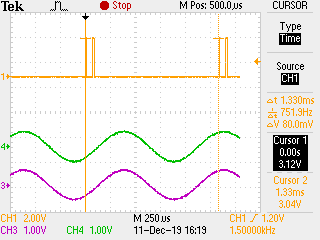
\includegraphics[width=0.6\linewidth]{FIR_Delay_Blocksize}
	\caption{Pulse zur Zeitmessung der Verarbeitungszeit. Die kleinen Pulse sind die Zeit zum Kopieren der rx-/tx-Buffer. Die kurze Lücke zwischen den Pulsen ist die Zeit für die Verarbeitung von zwei FIR Filtern mit je 11 Koeffizienten. Ausgangssignal L/R (grün/rot) 1kHz.}
	\label{pic:FIR_Delay_Blocksize}
\end{figure}

Die beiden kurzen Pulse in der Abbildung \ref{pic:FIR_Delay_Blocksize} entstehen durch den nachfolgend gelisteten Code in der Datei \texttt{dsp\_processing.c}.
Das Kopieren (Aufteilen in Links/Rechts) geschieht je ein Mal für die rxBuffer und die txBuffer, wobei ein Delay von $t_{Buffersplit}=16\mu\si{s}$ pro Kopiervorgang entsteht.
Die Abbildung \ref{pic:FIR_Delay_Blocksize} zeigt die Audiofunktion mit FIR-Filter. Im Falle der Verwendung einer Audio Passthrough Funktion beträgt die gesammte Verarbeitungszeit
inkl. Kopieren: $t_{delay}=40.8\mu\si{s}$. Daraus lässt sich schliessen, dass das Kopieren 
von rx in tx ohne weitere Verarbeitung nochmals ca. $f_{copy}=8\mu\si{s}$ benötigt.\\

\begin{lstlisting}[style=Cuvision, caption={GPIO togglen um die Kopierzeit zu messen}]
/* This Code takes 16 us for DSP_BUFFERSIZE_HALF = 64 and fCPU = 100MHz */
// copy sourceBuffer to leftSignalBuffer and rightSignalBuffer

HAL_GPIO_WritePin(LED1_GPIO_Port, LED1_Pin, GPIO_PIN_SET);

for (uint16_t index1 = 0; index1 < DSP_BUFFERSIZE_HALF; index1++) {
  rxLeft [index1] = (int16_t)(sourceBuffer[2*index1  ]);  
  rxRight[index1] = (int16_t)(sourceBuffer[2*index1+1]); 
}

HAL_GPIO_WritePin(LED1_GPIO_Port, LED1_Pin, GPIO_PIN_RESET);
\end{lstlisting}


\subsubsection{FIR Filter unterschiedlicher Anzahl Koeffizienten}

Theoretisch wird von einer FPU erwartet, dass diese ein FIR Filter mit der Effizienz von $1\frac{cycle}{TAP}$ mit Hilfe des Multiply-Accumulate Befehls (\texttt{MAC})) berechnet.
Bei ARM Cortex-M4 ist es jedoch so, dass das FIR Filter ohne Multiply-Accumulate Funktion kompiliert wird. Die Instruktion \texttt{VMLA.F32} benötigt 3 clock cycles \cite{ARM-M4-FPU-reference}. \\

\begin{lstlisting}[style=Cuvision,caption={Beispiel eines Multiply-Accumulate Befehls in C aus der CMSIS/DSP Library \texttt{arm\_fir\_f32.c}}, firstnumber=465]
acc3 += x4 * c0;
\end{lstlisting}

\begin{lstlisting}[style=Cuvision,caption={Assemblierte Multiply-Accumulate Instruktion aus obiger C-Code Zeile}]
0x080008E8 EE628A0D VMUL.F32 s17,s4,s26
0x080008EC EE766AA8 VADD.F32 s13,s13,s17
\end{lstlisting}

Die folgende Messung liefert das tatsächliche Ergebnis.

Mit dem Nachfolgenden Code wird die Verzögerung des FIR Filters bestimmt.
Der Versuch wird mehrmals mit unterschiedlicher Anzahl Koeffizienten durchgeführt.\\

\begin{lstlisting}[style=Cuvision,caption={GPIO togglen um FIR Verarbeitungszeit zu messen}]
HAL_GPIO_WritePin(LED1_GPIO_Port, LED1_Pin, GPIO_PIN_SET);

FIR_Filter_F32_Stereo(rxLeft, txLeft, rxRight, txRight);

HAL_GPIO_WritePin(LED1_GPIO_Port, LED1_Pin, GPIO_PIN_RESET);
\end{lstlisting}



\begin{table}[H]
	\centering
	\begin{tabular}{|c|c|c|c|}
		\hline
		\textbf{NUM\_TAPS} & \textbf{$t_{delay}$ {[}$\mu s${]}} & \textbf{clk cycles (@100MHz)} & \textbf{$\frac{\si{clk cycles}}{\si{TAP}}$} \\ \hline
		11                 & 63                      & 6'300                          & 4.47                       \\ \hline
		21                 & 103                     & 10'300                         & 3.83                       \\ \hline
		31                 & 148                     & 14'800                         & 3.73                       \\ \hline
		101                & 397                     & 39'700                         & 3.07                       \\ \hline
		251                & 937                     & 93'700                         & 2.92                       \\ \hline
	\end{tabular}
	\caption{Berechnungszeiten für zwei FIR Filter (Stereo) mit $n$ (\texttt{NUM\_TAPS}) Koeffizienten}
	\label{tab:FIR_performance}
\end{table}

\begin{equation}
\frac{clkcycles}{TAP}=\frac{f_{CPU}*t_{delay}}{2*NUM\_TAPS*BUFFERSIZE}
\end{equation}

\begin{equation}
\frac{clkcycles}{TAP}=\frac{100\si{MHz}*63\mu\si{s}}{2*11*64}=4.47
\end{equation}

\begin{figure}[H]
	\centering
	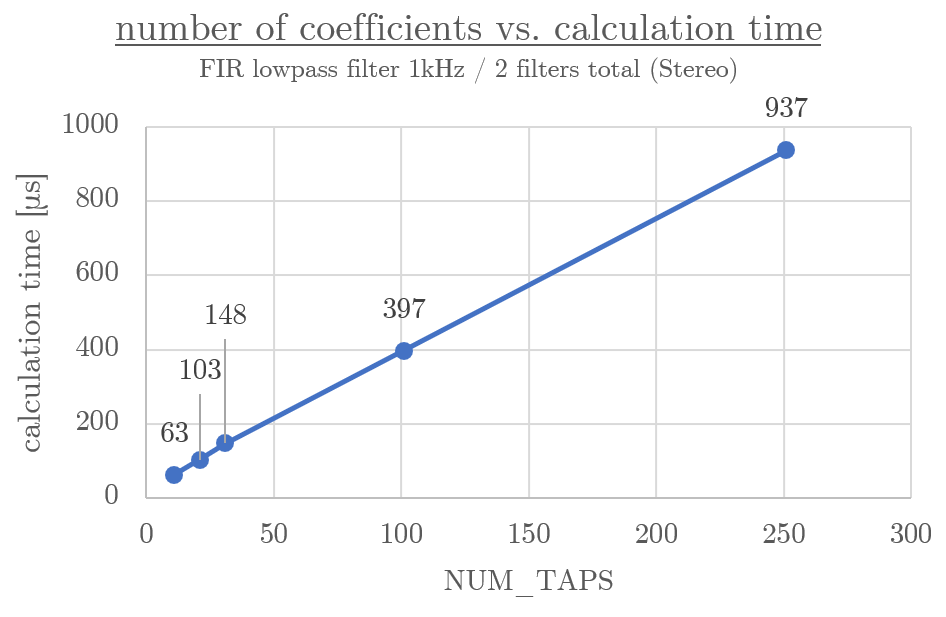
\includegraphics[width=0.8\linewidth]{FIR_NvsT}
	\caption{Die Daten aus Tabelle \ref{tab:FIR_performance} als Grafik dargestellt}
	\label{pic:FIR_NvsT}
\end{figure}

In der Tabelle \ref{tab:FIR_performance} und der Abbildung \ref{pic:FIR_NvsT} ist der Einfluss der Koeffizientenanzahl auf die Performance dargestellt.
Der Zusammenhang der Berechnungszeit und der Länge des Filters ist linear.
Bei der aktuellen Konfiguration mit der Buffergrösse und Samplingrate, können zwei FIR Filter also eine maximale Anzahl Filterkoeffizienten in der Nähe von $1'000$ haben, da sonst die kritische Verarbeitungsdauer von $t_{p}=1.333\si{ms}$ erreicht würde.

Die Abweichung um den Faktor 3 bis 4 in der Effizienz kann aktuell nicht erklärt werden.

\subsubsection{FFT Performance}

Hier wurde nur die FIR Performance behandelt. Relevant für die Beurteilung der FFT Performance ist das Whitepaper von ARM Limited \cite{ARM-Performance-Whitepaper}.

Gemäss den Zahlen im Whitepaper können mit einer Taktfrequenz von $f_{CPU}=100\si{kHz}$ auf einer Cortex-M4 Plattform folgende Werte erzielt werden.

\begin{table}[H]
	\centering
	\begin{tabular}{|c|c|c|}
		\hline
		\textbf{f32 FFT} & \textbf{delay {[}$\mu s${]}} & \textbf{$t_{delay}${[}$\mu\si{s}${]}} \\ \hline
		128              & 7000                & 70                             \\ \hline
		256              & 15000               & 150                            \\ \hline
		512              & 31000               & 310                            \\ \hline
		1024             & 56000               & 560                            \\ \hline
	\end{tabular}
	\caption{float32 FFT Performance auf Cortex-M4 mit 100MHz getaktet}
	\label{tab:FFT_performance}
\end{table}





